\chapter{Related work}

\section{Introduction}

In this chapter, we introduce a few related works and papers that align with concepts described in this dissertation. The language Elm for example describes in detail the challenges of functional reactive programming, tackling many of the same problems and describing similar solutions as encountered in FrDataFlow. Despite the similarities, the difference in platforms (Elm has to adhere to the limitations of the JavaScript execution engine in browsers, while FrDataFlow is constrained to the limits of the Racket runtime) has a significant impact on the potential to parallelization. 

\section{Reactive programming}

\subsection{Elm}

In 2012, Evan Czaplicki wrote his dissertation on Elm \citep{czaplicki_elm:_2012}, a functional reactive programming language for the web. In this paper, he presents a new language \textit{Elm} that supports concurrent functional programming for the web. Elm is compiled down to JavaScript using a compiler written in Haskell and promises to produce no runtime errors when everything compiles. 
Most of the reactive programming concepts in FrDataFlow were actually heavily inspired by Elm, such as \textit{signals} and the \textit{lift} function. 
Another concept inspired by Elm is signal graphs: reactive primitives as nodes and value flows as edges. Of course, source signals are a bit different in the web. For example, Elm provides source signals that represent mouse clicks, mouse positions or generally any kind of DOM event which is captured by the standard library. In the isolated, experimental little world of FrDataFlow, primitive source signals other than the current time were hard to come by. 

\subsubsection{Order of events}

Looking at a signal graph, it is easy to imagine the parallel execution of the nodes. However, the order of events is very important. 
Take for example the signal graph shown in figure \ref{fig:relatedwork-elm-eventsorder}.

\begin{figure}[h!]
	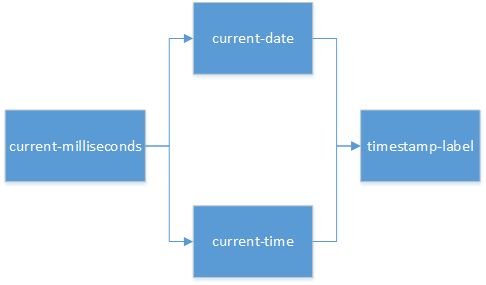
\includegraphics[width=\textwidth]{images/RelatedWork-Elm-EventsOrder.png}
	\caption{The current timestamp is based on two different computations of \textit{current-milliseconds}}
	\label{fig:relatedwork-elm-eventsorder}
\end{figure}

If a new value appears for current-milliseconds (the number of milliseconds since 1 Jan 1970), we compute the current date and current time separately, to combine these two data points into a single label called \textit{timestamp-label}. Imagine now that the computation of the current time takes significantly longer than the computation of the current date. In fact, we can contemplate that the derivation of the time would actually need to derive the date first, and then use the remaining milliseconds from midnight to determine the time. Of course, depending on the date and the timezone, this could result in different clock times.
This leads us to conclude that the calculation of \textit{current-time} is slower than \textit{current-date}. 

Now imagine that these computations are run in parallel and that their outputs are piped to the timestamp label as fast as the hardware allows it. If the date is so much faster to process, it becomes possible that the timestamp label starts receiving more than one \textit{current-date} for every \textit{current-time}, leading to situations where the date and time that are shown do not both trace back to the same value of \textit{current-milliseconds} they were derived from. 

In Elm, this problem was fixed by the introduction of a global event dispatcher, which imposes a few constraints on the signal graph update loop:

\begin{itemize}
	\item Signals with more than one parent must wait for all parents to produce a value before recomputation happens. This is the same approach taken in FrDataFlow. 
	\item When source signals emit a new value, all nodes receive that event and pass forward a "nothing changed" notification. In FrDataFlow, the approach is to simply push the current value. 
\end{itemize}


\subsubsection{Parallelization}

In Elm, the constraints of the platform are slightly different. The JavaScript runtime does not really provide native parallelization\footnote{Web workers exist, which were designed offload work in background threads. However, they come with two rather expensive limitations, the first being that messages between workers must be primitive data types, so there is no support for passing along functions with closures, only simple messages such as strings or numbers. Secondly, these web workers directly map to operating system threads, making them quite expensive to set up and tear down. The end result is that these workers are not a good fit for the small, atomic computations we are dealing with in reactive nodes.}, so while the language itself could perfectly support parallelism, unfortunately its platform does not. 

Elm does provide some workarounds for when the synchronous nature of its node processing causes performance bottlenecks, namely asynchronous updates. This keyword decouples a subset of the graph from the main graph and allows it to update independently, avoiding the situation where it would have to wait for long running synchronous updates. However, this is still purely a data correctness and timing feature and unfortunately does not tackle the lack of parallelization support.

In fact, the paper does mention a possible solution to run Elm programs in parallel: if closures can be avoided somehow (for example by compiling to an intermediate language which explicitly lists the used captured variables) and if functions are passed as strings (and then dynamically interpreted inside the workers), web workers could technically provide a parallel execution mechanism. It was not considered worthwhile though, because of the amount of overhead to orchestrate this and the possible security ramifications.

\subsection{FrTime}

Another project that is closely related to FrDataFlow is \textit{FrTime}. This is a reactive programming language that implicitly implements signals for primitive operators. The idea is that applications written in regular Scheme could be switched over to FrTime to introduce reactive programming without having to rewrite the code. Contrary to FrDataFlow, expressions in FrTime do not require explicit use of the lift operator, but are implicitly used when any of the primitive operators are used. For full effect, FrTime provides a REPL (Read Eval Print Loop) console which takes expressions and immediately prints the result. There is an extra feature though: values which are signals keep getting updated in the history. When for example the plus operator is applied to a fixed number and the current seconds, this creates a signal which continuously updates with the result, inside the console. Rather than evaluating the expression and returning a signal like in FrDataFlow, FrTime immediately returns a value and keeps updating that value, even inside the REPL history. 

\begin{lstlisting}[caption={REPL in FrTime},captionpos=b,label={lst:relatedwork-frtime-repl}]
> seconds 			
1496651429
> (even? seconds) 
#f
> (+ 10 seconds)
1496651439
\end{lstlisting}

See the listings \ref{lst:relatedwork-frtime-repl} and \ref{lst:relatedwork-frtime-repl-5s}. In the first sample, some commands are entered into the REPL and their output is shown below each command.
Note that the listing \ref{lst:relatedwork-frtime-repl-5s} simply shows exactly the same screen from listing \ref{lst:relatedwork-frtime-repl} but 5 seconds later. It is not revealed to the user that the expressions he is using are built with signals that update in the background. It only becomes clear, as time goes by, that these values automatically update in the REPL.

\begin{lstlisting}[caption={REPL in FrTime, 5 seconds later},captionpos=b,label={lst:relatedwork-frtime-repl-5s}]
> seconds
1496651434
> (even? seconds)
#t
> (+ 10 seconds)
1496651444
\end{lstlisting}

\subsubsection{Push-driven evaluation}

A major difference between FrTime and FrDataFlow is its update model. FrDataFlow implements what is called a push driven evaluation. This means that parent signals - or producers, as FrTime calls them - have references to their children (dependents in FrTime). When a parent signal gets updated, it can follow along the edges of its dependencies to ripple the change forward in the graph. Since child signals do not hold references to their parents, closures are used during the signal construction process to capture references to these parents in the callback procedure.

In FrDataFlow, callbacks and closures are not an essential part of the update mechanism. All signals are stored in a topologically sorted graph, where each signal can access its parents and children. When a new value propagates through the graph, the update loop simply grabs the necessary information from the parent signals to provide to the child.

FrTime's callback model in combination with their queue based update algorithm actually comes with a string of performance problems, which they try to address by \textit{lowering} \cite{burchett_lowering:_2007} their operators, essentially collapsing multiple operations into one to reduce overhead and to minimize the graph size. Although this considerably improves execution time, it unfortunately also reduces parallelization opportunities by growing the size of one signal node. 


\section{Dataflow Model}

\subsection{title}



